\section{Optimization}
\label{sec:optimization}

This section addresses three performance challenges: How to use shared memory and RDMA efficiently? How to achieve socket-compatible zero copy? How to avoid thread wakeup cost when multiple threads share a CPU core?

\subsection{High Performance Queue}
\label{subsec:lockless-queue}

\begin{figure}[t]
	\centering
	
\includegraphics[width=0.4\textwidth]{images/fixme.pdf}
	\vspace{-5pt}
	\caption{Performance comparison of queues.}
	\vspace{-10pt}
	\label{fig:queue-performance}
\end{figure}

%We first revisit requirements of the queue between a pair of communicating threads in different applications or hosts. A sender enqueues messages sequentially. At the same time, a receiver peeks and dequeues messages at any position. The message may be a control command or data of a FD, so the message size is variable.
%Our aim is high throughput and low latency when messages in the queue are dequeued in the same order as enqueued, and preserve liveness when dequeuing in arbitrary order.
Shared memory and RDMA are state-of-the-art methods for inter-core and inter-host communication.
However, as Figure~\ref{fig:queue-performance} shows, sharing \emph{head} and \emph{tail} pointers between sender and receiver introduces inter-core cache migration overheads in shared memory and unacceptable latency for RDMA.
For high throughput and low latency, our principle is that each shared memory region is either writable by the sender or receiver, but never both.
Because the receiver needs to modify \emph{isdel} and \emph{nextptr} fields, we create a \emph{shadow ring buffer} in receiver's private memory and update the corresponding offset in place of shared memory.

\parab{Credit-based ring buffer.}
%Most ring buffer designs share \textit{head} and \textit{tail} pointers between sender and receiver, which introduces an additional cache migration or RDMA operation. To eliminate such overhead, we keep \textit{head} and \textit{tail} pointers locally in sender and receiver respectively.
To tell whether the ring buffer is full, the sender maintains a \textit{credits} count, indicating the number of free bytes in ring buffer. When sender enqueues a message, it consumes a credit. When receiver dequeues a message, it increments a counter locally, and writes a \textit{credit return flag} in sender's memory once the counter exceeds half the size of ring buffer. The sender regains credits upon detecting the flag.

\parab{Enqueue and dequeue.}
Sender enqueues message at \textit{tail} pointer. For shared memory queue, first, sender clears header of the next message to prevent the receiver from considering junk data in the ring buffer to be a message. Next, sender writes payload, then writes header, finally advances \textit{tail}. Receiver polls \textit{isvalid} at \textit{head} pointer, then copies the message, finally advances \textit{head}.
For RDMA, the sender maintains a local copy of ring buffer, and we use one-sided RDMA write to synchronize updates from sender to receiver.
%For RDMA, it is known that one-sided verbs has higher throughput than two-sided ones; short messages has lower throughput than large ones~\cite{kalia2014using,kaminsky2016design}.
%In light of this, the inter-host queue has two identical copies in pinned sender and receiver memory, and we use one-sided RDMA write to synchronize updates from sender to receiver.
%\libipc{} polls CQ to limit the number of in-flight (sent but not acknowledged) messages, which is not only required by RDMA NIC, but also enables \emph{adapative batching}~\cite{li2016clicknp,li2017kv}.
%When a message is enqueued to the ring buffer and the RDMA send queue is not full, it is immediately sent as an RDMA message.
%When \libipc{} polls CQ and finds an empty slot in send queue, it sends all queued but unsent data in queue as an RDMA message, because the messages are stored back-to-back in the queue.


\parab{Consistency between payload and metadata.}
One may think that out-of-order execution may mandate the use of memory fence instructions. Actually, memory fence is unnecessary. For shared-memory queue, X86 processors from Intel and AMD provides total store ordering~\cite{sewell2010x86,intel-manual}, which implies that two writes are observed by other cores in the same order as they were written. An 8-byte \texttt{MOV} instruction is atomic, so writing a header is atomic. Because sender writes header after payload, the receiver would read a consistent message after polling \textit{isvalid} flag.
Because RDMA does not ensure write ordering within a message~\cite{infiniband2000infiniband}, sender uses \textit{RDMA write with immediate} verb to generate completions on receiver. The receiver polls RDMA completion queue rather than the ring buffer. RDMA ensures cache consistency on receiver, and the completion is guaranteed to be delivered after writing the data.


\parab{Amortize polling overhead.}
Polling queues wastes CPU cycles of the receiver when a pair of threads do not communicate frequently. To this end, we amortize polling overhead using two techniques.
For RDMA queues, we leverage the RDMA NIC to multiplex event notifications into a single queue.
A thread uses a \textit{shared completion queue} for all RDMA connections, so it only needs to poll one queue rather than multiple queues.
For shared memory queues, each queue can switch between \textit{polling} and \textit{interrupt} modes. The queue to the monitor is always in polling mode. Receiver of each queue maintains a counter of consecutive empty polls. When it exceeds a threshold, the receiver sends a notification to sender and stops polling after a while. When sender writes to a queue in interrupt mode, it also notifies the monitor and the monitor will signal the receiver to resume polling.


\subsection{Zero Copy}
\label{subsec:zerocopy}

\begin{figure}[t]
	\centering
	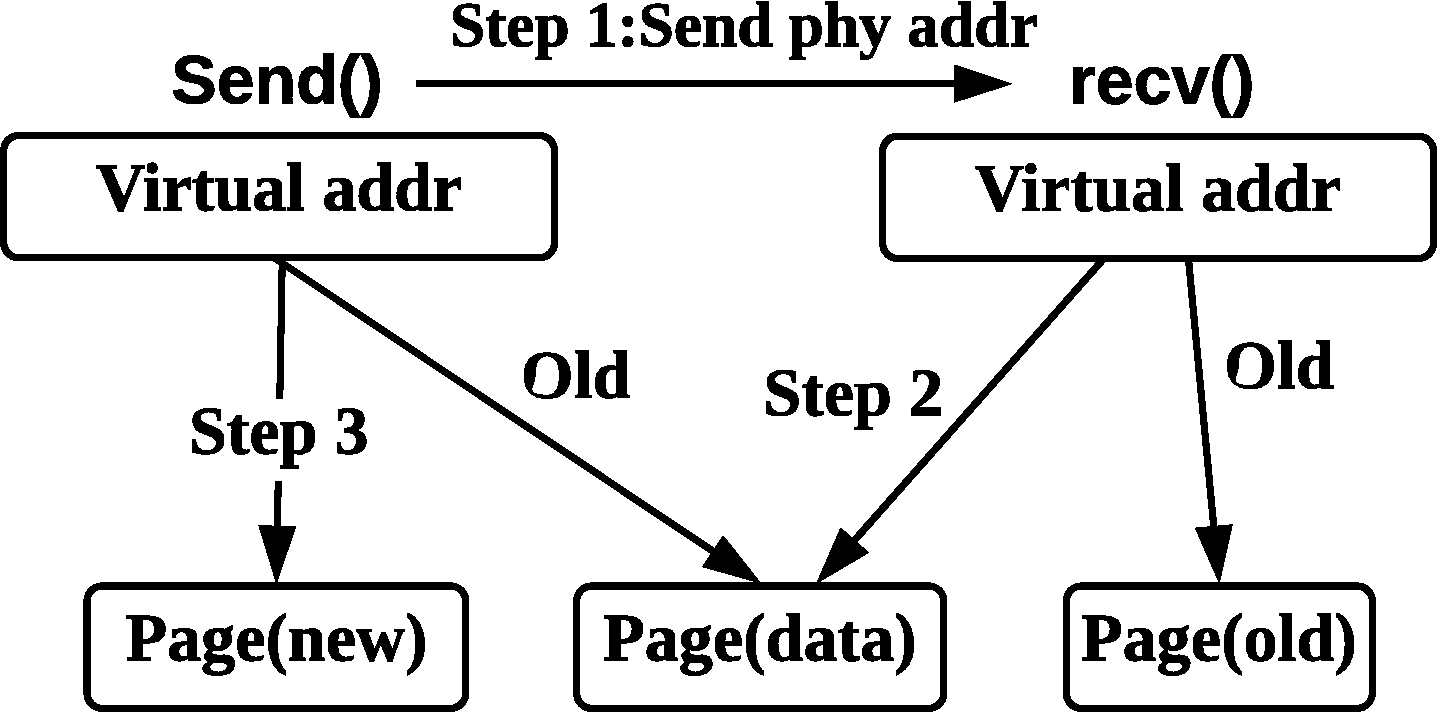
\includegraphics[width=0.3\textwidth]{images/zerocopy}
	\caption{Zero copy via page remapping. Step 1: \texttt{send}, sender get physical address and send via shared memory. Step 2: \texttt{recv}, receiver maps the page to buffer. Step 3: sender remaps buffer on memory write.}
	\vspace{-15pt}
	\label{fig:zerocopy}
\end{figure}

The main challenge for zero copy is to maintain the semantics of socket API, as discussed in Sec.\ref{subsec:performance-challenges}.
%A sender may write the send buffer after non-blocking \texttt{send}, and the receiver does not know the receive buffer before \texttt{recv}.
Fortunately, virtual memory provides a layer of indirection, so we can remap virtual address of a buffer to another physical page if the data occupies entire 4~KiB pages.
We wrap around \texttt{malloc} and \texttt{realloc} functions and allocate 4~KiB aligned addresses for large allocations, so most buffers will align to page boundary.
If the size of send message is not a multiple of 4~KiB, the last chunk of data is copied on \texttt{send} and \texttt{recv}.

\subsubsection{Zero Copy for Intra-Server Socket}
\label{subsec:zero-copy-intra}

\parab{Page remapping.}
As shown in Figure~\ref{fig:zerocopy}, for \texttt{send} operation that is aligned to page boundary and at least 8~KiB, \libipc{} invokes the kernel to get encrypted physical page addresses of send buffer and send the pages to receiver via shared memory queue.
The address is encrypted to prevent unsolicited mapping of arbitrary pages.
Because the sender may read the buffer after \texttt{send} or send the buffer to multiple receivers, the physical page cannot be remapped.
Additionally, \texttt{send} needs to write-protect the buffer because the receiver needs to read it.
On the receiving side, \libipc{} invokes the kernel to remap the encrypted physical pages to the application-provided receive buffer.
\texttt{recv} also needs to write-protect the buffer.

\parab{Minimize copy-on-write.}
A challenge arises when sender writes the buffer after \texttt{send}.
Existing zero-copy socket designs~\cite{thadani1995efficient,chu1996zero} use copy-on-write. %Copy is required because the sender may read the non-written part of the page.
Because most applications reuse the buffer for subsequent send operations, copy-on-write is invoked in most cases, making zero-copy essentially useless on sender.
Our observation is that most applications overwrite entire pages of the send buffer via \texttt{recv} or \texttt{memcpy}. %so it is unnecessary to copy old data when the first byte of the page is written.
Zero-copy by \texttt{recv} already remaps the buffer without triggering copy-on-write.
We add preamble code to \texttt{memcpy} in both \libipc{} runtime and compiler inline library. 
For page-aligned copy to \libipc{} buffers, the preamble code invokes the kernel to remap new pages and disable write protection.

\parab{Page pool in user space.}
A second challenge is that page remapping requires the kernel to allocate and free pages for each \texttt{send} and \texttt{recv}. Page allocation in kernel acquires a global lock, therefore it is inefficient. Instead, \libipc{} manages a pool of free pages in each process.
\libipc{} also tracks the origin of received zero-copy pages.
Whenever a page is remapped, if it is from another process, \libipc{} sends a message to the original process to return the pages.

\subsubsection{Zero Copy RDMA}
\label{subsec:zero-copy-rdma}

On sender, zero copy RDMA is similar to intra-server. We use physical addresses in RDMA verbs to eliminate memory registration and address translation overhead, as recommended by NIC documentation~\cite{mellanox-zerocopy}. The page containing send data is freed after RDMA completion. On receiver, \libipc{} prepares a page pool during initialization. The sender manages the pool. Upon \texttt{send}, sender allocates pages from the pool to determine the remote address of RDMA write, and send the physical address via ring buffer. Upon \texttt{recv}, \libipc invokes the kernel to map physical pages in the ring buffer message to application buffer address. When the pages are remapped, \libipc{} returns the pages to the pool in sender via RDMA.
%For security, kernel validates that page numbers are in the huge-page receive buffer.

%\subsubsection{Zero Copy TCP}
%\label{subsec:zero-copy-tcp}
%
%For TCP connections, we optimize the user-space TCP/IP stack to remove memory copy between \libipc{} and NIC.
%Because the payloads of sent and received packets need to align at 4~KiB page boundary, we leverage scatter-gather support in modern NICs~\cite{mellanox} to separate packet header from application payload.
%%During initialization, \libipc{} queries IP and Ethernet MAC address from the kernel and constructs a packet header template.
%For \texttt{send}, \libipc{} constructs a packet header to a NIC send work request, then fills in the payload buffer address from application. 
%For receiving data, in background, \libipc{} issues NIC receive work requests with a 54-byte buffer to store Ethernet, IPv4 and TCP headers, followed by a page-aligned buffer to store payload.
%%In corner cases where the received header length is not 54 bytes, \libipc{} reassembles the packet.
%Upon \texttt{recv}, the payload buffer is remapped to application.

\subsection{Cooperative Multitasking}
\label{subsec:process-mux}

To deal with the scenario where multiple threads share a CPU core, rather than using OS event notification, we use cooperative multitasking to switch thread contexts efficiently on a CPU core.


\parab{Event notification.}
To minimize context switch, \sys{} runs in user mode and uses cooperative multitasking to multiplex processes on CPU cores. Coordination and delegation based on message passing also requires processes to respond to messages promptly. However, processes may execute application code without calling \libipc{} for a long time. To tackle this issue, we design a \textit{signal} mechanism analogous to interrupts in operating systems. Event initiators  first poll the receive queue for a period of time for ack. If no reply, it sends a Linux \texttt{signal} to the receptor and wake up the process.

The signal handler, registered by \libipc{}, first determines whether the process is executing application or \libipc{} code. To determine this, \libipc{} sets and clears a flag at entry and exit of the library. If signal handler finds that the process is in \libipc, it does nothing and \libipc{} will process the event before returning control to the application. Otherwise, the signal handler immediately processes messages from the emergency queue to the monitor, then return control to the application. 
%Because \libipc{} is designed to be fast and non-blocking, message passing initiators will soon receive the response.

\parab{Polling and sleep.}
When an application calls non-blocking socket operations, \libipc{} polls queues of the specified FD and the emergency queue to the monitor, then returns immediately. For blocking operations (\textit{e.g.} blocking \texttt{recv}, \texttt{connect} and \texttt{epoll\_wait}), \libipc{} first polls the queues once. If the operation is not completed, \libipc{} calls \texttt{sched\_yield} to yield the processor to other processes on the same core. %As stated in Sec.~\ref{subsec:bottleneck}, context switch in cooperative multitasking only takes 0.4~$\mu$s. However, an application may wait a long time for an external event, making frequent wake-ups wasteful. In this regard, we count consecutive wake-ups which does not process any message, and puts the process to sleep when this reaches a threshold. 
If \libipc{} continues to yield for a certain number of rounds, it will put itself into sleep. Before sleeping, it sends a message to the monitor and all peers, so they can wake up the sleeping process after sending a message via shared-memory queue.

\parab{Handling events from kernel.}
An application needs to poll kernel FDs (\textit{e.g.} files and semaphores) together with socket FDs.
\libipc{} creates a per-process \textit{epoll thread} to poll kernel FDs for all application threads. When it receives a kernel event, it broadcasts the event to application threads via shared memory queues.%\texttt{Epoll\_wait} in \libipc{} will return such kernel events in addition to socket events. Note that Linux allows an event to be received by multiple threads sharing the FD.

%\parab{Exit.}
%When a process exits, the \texttt{atexit} handler of \libipc{} notifies the monitor and all peers to close connections and mark the queues as dead. However, a process may crash or get killed. In this case, monitor detects process death via \texttt{SIGHUP} of the bootstrap socket (Sec.~\ref{subsubsec:fork_fork}) and notify its peers. When a process switches to \texttt{daemon} mode or \texttt{execve} another program, it first follows the process exit procedure, then calls the system call. After that, \libipc{} is re-initialized.
